\section{Data Approximation}
\label{sec-data}






Big data has large volume, and, hence, the space complexity of big data analytic tasks starts raising more concerns.
Given a class $Q$ of queries on a data set $D$, data approximation is to transform $D$ into a smaller data set $D'$ such that $Q$ on $D'$ returns a satisfiable approximate answer in a more efficient way. Further, it is typically common that query $Q$ needs to be (slightly) modified to $Q'$ to accommodate  the changes of $D$ to $D'$, as shown in Fig.~\ref{fig-tech-dataappro}. Similar to query approximation, data approximation needs to reach a balance between the query efficiency and answer accuracy.


The rationale of data approximation has roots in the Pareto principle\footnote{\small \url{https://en.wikipedia.org/wiki/Pareto_principle}} that ``states that, for many events, roughly 80\% of the effects come from 20\% of the causes''. The critical thing for data approximation is to determine which part of data is relevant to tasks (belong to the 20\%).
 By this principle, for many big analytic tasks, one may only need to keep a small amount of the data to derive ``satisfiable'' answers.
For example, when we are to build a predictive model on the stock of razers for an online store based on the order history of customers, orders from men are good enough. While on the stock of lipsticks, those from women are good enough. That is to say,  it is not necessary to use the entire data for certain data analytic tasks.



However, it should be pointed out that there are data analytic tasks such that data approximation could not work well. For example, an online store needs to count the total number of goods in its catalog.  Essentially the entire goods should be considered for this task, and if a (small) portion of goods are chosen, it is hard to have a ``satisfiable'' result.


We next explain data approximation computation in more detail with three different data analytic tasks.



\stitle{(2) Proxies for Shortest Paths/Distances~\cite{MaFLWCH16}}


We study the {\em node-to-node shortest path} ({\em distance}) problem on large graphs: given a weighted undirected graph $G(V, E)$ with non-negative edge weights, and two nodes of $G$, the source $s$ and the target $t$, find the shortest path (distance) from $s$ to $t$ in $G$.
The Dijkstra's algorithm with Fibonacci heaps runs in $O(n\log n + m)$ due to Fredman \& Tarjan~\cite{CormenLRS01}, where $n$ and $m$ denote the numbers of nodes and edges in a graph, respectively, which remains asymptotically the fastest known solution on arbitrary undirected graphs with non-negative edge weights.
%The challenge of computing shortest paths on large graphs.
However, computing shortest  paths and distances remains a challenging problem, in terms of both time and space cost, on large-scale graphs. Hence, various optimizations have been developed to speed-up the computation.

To speed-up shortest  path and distance queries, our approach is to use {\em representatives}, each of which captures a set of nodes in a graph. The task of finding a proper form of representatives is, however, {\em nontrivial}. Intuitively, we expect representatives to have the following properties.
%
(1) A small number of representatives can represent a large number of nodes in a graph;
%
(2) Shortest paths and distances involved within the set of nodes being represented by the same representative can be answered efficiently; And,
%
(3) the representatives and the set of nodes being represented can be computed efficiently.

\stitle{1. Preprocessing}. Given graph $G(V, E)$, the preprocessing module executes the following.

\sstab (1) It first computes all \dras and their maximal proxies with a linear algorithm, referred to as  $\compDRAs$ \cite{journal-version2016}.

\sstab (2) It then pre-computes and stores all the shortest paths and distances between any node in a \dra and its proxy.
%
To support shortest distance queries, for each node in a \dra, we store its proxy $u$, its distance to $u$ and the component of $A^{+}_u$ to which it belongs,
and to support shortest path queries, we further keep the shortest paths from proxy $u$ to all nodes in the \dra.

\sstab (3) It finally computes the reduced subgraph $G'$ by removing all \dras, but keeping their proxies, from graph $G$.


\stitle{2. Query answering}. Given two nodes $s$ and $t$ in graph $G(V$, $E)$  and the pre-computed information, the query answering module executes the following.


\sstab (1) When nodes $s$ and $t$ belong to the same \dra $G[A^+_u]$ with proxy $u$ such that $A^+_u$ = $A^1_u\cup\ldots A^h_u$.

If $s$ and $t$ further fall into the same component $A^i_u$ ($i\in[1,h]$), it invokes the Dijkstra's algorithm on the subgraph $G[A^i_u]$ to compute the shortest path and distance between $s$ and $t$. Otherwise, it simply returns $\path(s, u)/\path(u, t)$ or $\dist(s, u)$ + $\dist(u, t)$ in constant time.

\sstab (2)  When $s$ and $t$ belong to two \dras $G[A^+_{u_s}]$ and $G[A^+_{u_t}]$ with proxies $u_s$ and $u_t$, respectively.

 As shown in Section~\ref{sec-proxy}, we know that $\path(s, t)$ = $\path(s, u_s)/$ $\path(u_s, u_t)/$ $\path(u_t, t)$, in which $\path(s, u_s)$ and $\path(u_t, t)$ are already known. Hence, it simply invokes an algorithm (\eg~\arcflag \cite{MohringSSWW05}, \tnr~\cite{bast2014route}, \ah~\cite{zhu2013shortest}) on the reduced graph $G'$ for computing $\path(u_s, u_t)$.
%
Similarly, it computes $\dist(s, t)$ = $\dist(s, u_s)$ + $\dist(u_s, u_t)$ + $\dist(u_t, t)$.


We have studied how to speed-up (exact)  shortest path and distance queries on large weighted undirected graphs.
To do this, we have proposed  a light-weight data reduction technique, a notion of proxies such that each proxy represents a small subgraph, referred to as \dras, and proxies and \dras can be computed efficiently in linear time.  We have also verified,
both analytically and experimentally, that proxies significantly reduce graph sizes and improve efficiency of existing methods.


\begin{figure}[tb!]
  \vspace{-1ex}
  \begin{center}
  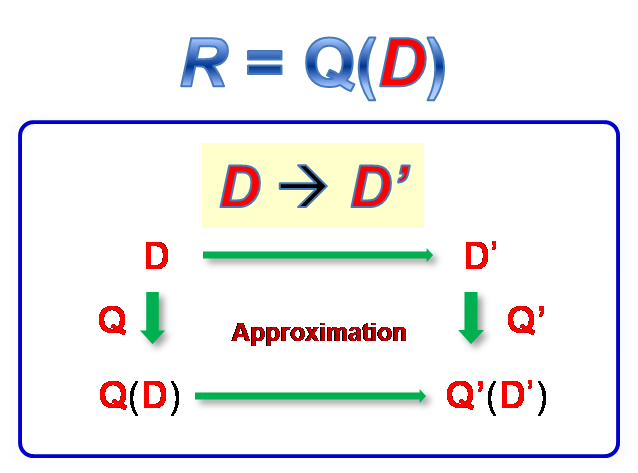
\includegraphics[scale=0.45]{./dataApprox.png}
  \end{center}
  \vspace{-3ex}
  \caption{Data approximation}\label{fig-tech-dataappro}
  \vspace{-2ex}
\end{figure}

\stitle{(3) Ensemble Enabled Link Prediction~\cite{DuanMAMH17}}

The problem of {\em link prediction} or {\em link inference} is that of predicting the formation of future links in a dynamic and
evolving network. The link prediction problem has numerous
applications, such as the recommendation of friends in a social
network, the recommendation of images in a multimedia network, or
the recommendation of collaborators in a scientific network, therefore, link
prediction methods have been extensively studied  because of their numerous applications in various network-centered domains.


Link prediction methods are often applied to very large networks, which are also sparse.  The massive sizes of such networks can
create challenges for the prediction process in spite of their sparsity. This is because the {\em search space} for the link
prediction problem is of the size $O(n^2)$, where $n$ is the number of nodes. Quadratic scalability can rapidly become untenable for
larger networks. In fact, an often overlooked fact is that most {\em current link prediction algorithms evaluate the link
propensities only over a subset of possibilities rather than exhaustively search for link propensities over the entire network}, \eg \cite{dwang,lee,zhao2016,zhu2016}.


In order to understand why this is the case,
consider a network with $10^6$ nodes. Note that a size such as
$10^6$ is not large at all by modern standards, and even common
bibliographic networks such as DBLP now exceed this size. Even
for this modest network, the number of {\em possibilities} for links
is of the order of $10^{12}$. Therefore, a 1GHz processor would
require at least $10^3$ seconds just to allocate one {\em machine cycle} to
every pair of nodes. This implies that in order to determine the
top-ranked link predictions over the {\em entire network}, the
running time will be much larger than $10^3$ seconds.  It is
instructive, therefore, to examine how this (lower bound on) running
time scales with increasing network size. Table~\ref{time} shows the
time requirements for allocating a single machine cycle to each
pair-wise possibility. The running time in this table represent
very optimistic lower bounds on the required time because link
prediction algorithms are complex and require far more than a single
machine cycle for processing a node-pair. Note that for larger
networks, even the presented lower bounds on the running time are
impractical.
\begin{table}
\caption{The $O(n^2)$ problem in link prediction: Time required to
allocate a {\em single machine cycle} to every node-pair possibility
in networks of varying sizes and processors of various speeds.}
\label{time}
\vspace{0ex}
\centering
\begin{tabular}{cccc}
\hline \hline Network Sizes & 1 GHz &  3 GHz & 10 GHz \\
\hline \hline $10^6$ nodes & 1000 sec. & 333 sec. & 100 sec.\\
\hline $10^7$ nodes & 27.8 hrs &  9.3 hrs &  2.78 hrs\\
\hline $10^8$ nodes & $>100$ days &  $>35$ days & $> 10$ days\\
\hline $10^9$ nodes & $>10000$ days & $>3500$ days & $> 1000$ days\\
\hline \hline
\end{tabular}
\vspace{-2ex}
\end{table}


It is noteworthy that most link prediction algorithms in the
literature are not designed to search over the entire space of
$O(n^2)$ possibilities. A closer examination of the relevant
publications shows that even for networks of modest size, these
algorithms perform benchmarking  only by evaluating over a {\em
sample of the possibilities} for links. This is only to be expected
in light of the lower bounds shown in Table~\ref{time}.  In other
words, the {\em complete ranking problem} for link prediction in
very large networks remains largely unsolved at least from a
computational point of view. It is evident from the presented lower
bounds in Table~\ref{time} that any ranking-based link prediction
algorithm {\em must integrate search space pruning} within the
prediction algorithm in order to even  have any  hope of exploring
the $O(n^2)$ search space in a reasonable amount of time. The
algorithmic design of most link prediction algorithms largely
overlooks this basic requirement~\cite{chancc,propflow}.



To this end, we explore an {\em ensemble approach} to
achieving the aforementioned goals.

We show how to make latent factor models
practical for link prediction by decomposing the search space into a
 set of smaller matrices. As a result, large parts of the $O(n^2)$
search space can be pruned without even having to evaluate the
relevant node pairs. An optimizing method is also provided for
speeding up the search process when a threshold is available.
This provides an efficient approach for the
top-$k$ problem in link prediction.

Furthermore, our problem
decomposition method is an ensemble approach enabled with three
structural bagging methods with performance guarantees, which has obvious {\em
effectiveness} advantages. By incorporating with the characteristics of  link prediction, the bagging methods maintain high prediction
accuracy while reducing the network size via graph sampling techniques.
Note that the same bias-variance
tradeoffs apply to the link-prediction problem, as they apply to the
standard classification problem. Therefore, the use of an ensemble
approach has obvious effectiveness advantages as well.


Using real-life datasets, we finally conduct an extensive experimental study, and show that our ensemble approach for link prediction is both effective and efficient.



\eat{
\stitle{(1) Network Anomaly Detection~\cite{HuAMH16}}
We have adopted the idea in the process of dealing with large graphs in the study of anomaly detection in graph streams, when dealing with the matrix representation of a social graph, and  we have both theoretically and experimentally shown that simplifying the matrix by replacing a part of small entry values  with zero has few affects on the computation of eigenvectors~\cite{YuAMW13}.
}%%%%%%%%%%%%EAT






